\begin{figure}[h!]
\begin{center}
% \vspace{-15pt}
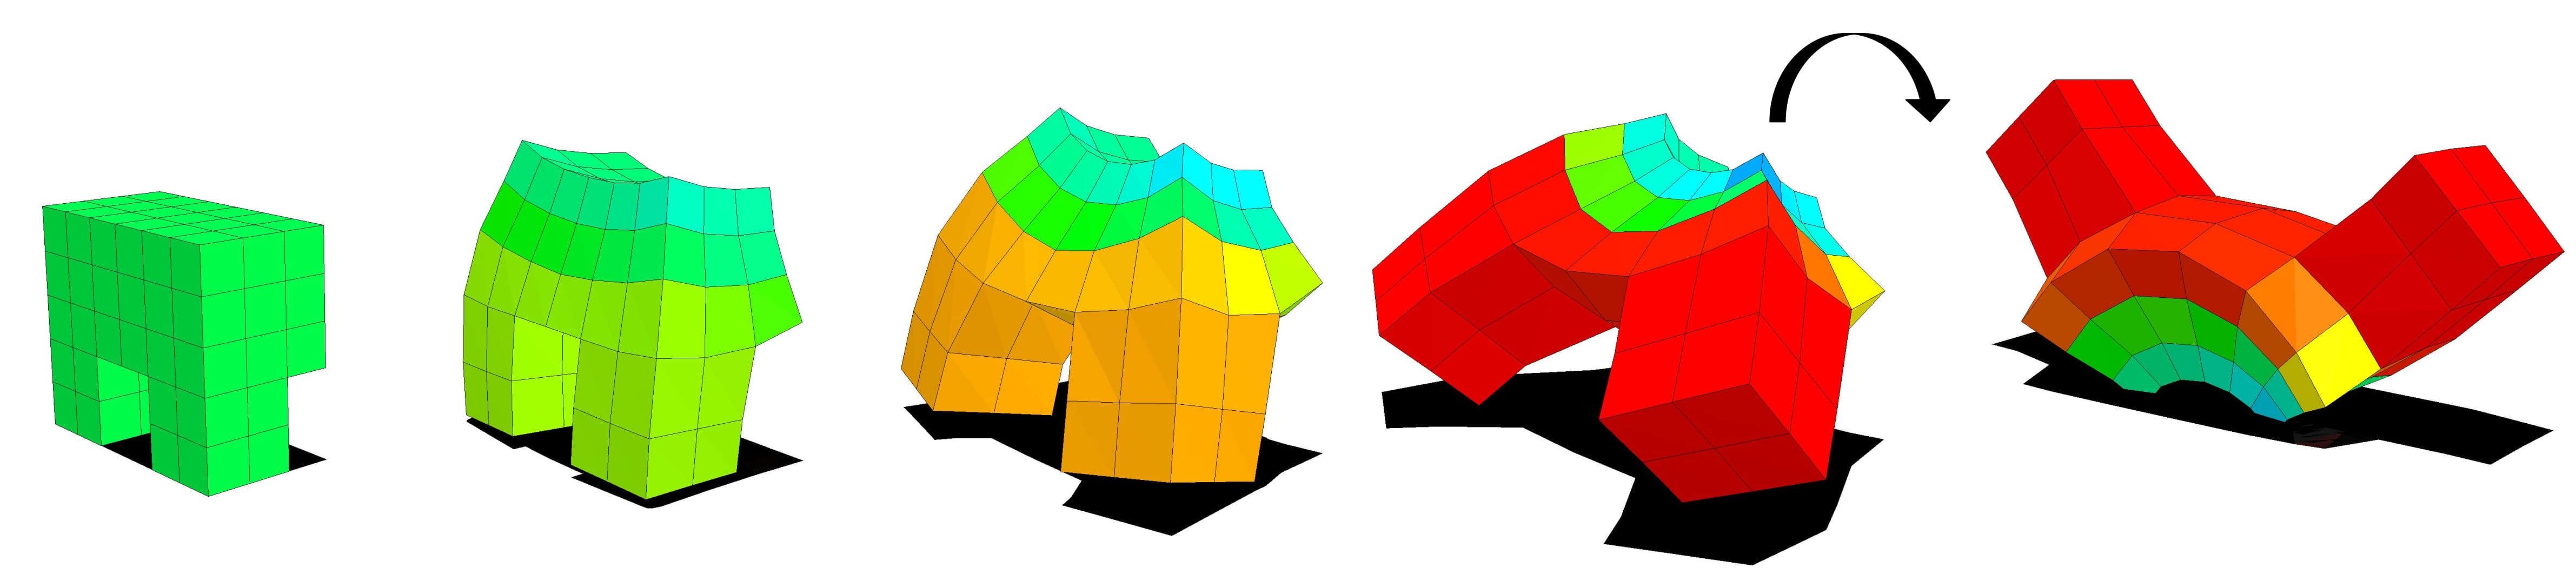
\includegraphics[trim={0 0 0 0},clip,width=\linewidth]{Chapter05/fig/Flipper2.jpg}\\
% \vspace{-5pt}
\caption{\label{fig:flipper}
This damaged robot (amp.~=~1/2~body) contracted its spine, expanded its limbs, and flipped over onto its back to walk lengthwise and exploit the elastic properties of its new arms
(\href{https://youtu.be/WwYdSnuJBBA}{\textcolor{blue}{\textbf{\texttt{youtu.be/WwYdSnuJBBA}}}}).
}
\vspace{-1em}
\end{center}
\end{figure}